% This is a LaTeX thesis template for Monash University.
% to be used with Rmarkdown
% This template was produced by Rob Hyndman
% Version: 6 September 2016

\documentclass{monashthesis}

%%%%%%%%%%%%%%%%%%%%%%%%%%%%%%%%%%%%%%%%%%%%%%%%%%%%%%%%%%%%%%%
% Add any LaTeX packages and other preamble here if required
%%%%%%%%%%%%%%%%%%%%%%%%%%%%%%%%%%%%%%%%%%%%%%%%%%%%%%%%%%%%%%%

\author{Beinan Xu}
\title{What makes a good prediction interval or probabilistic forecast?}
\studentid{26401746}
\def\degreetitle{Masters of Applied Econometrics}
% Add subject and keywords below
\hypersetup{
     %pdfsubject={The Subject},
     %pdfkeywords={Some Keywords},
     pdfauthor={Beinan Xu},
     pdftitle={What makes a good prediction interval or probabilistic forecast?},
     pdfproducer={Bookdown with LaTeX}
}


\bibliography{thesisrefs}

\usepackage{amsthm}
\newtheorem{theorem}{Theorem}[chapter]
\newtheorem{lemma}{Lemma}[chapter]
\theoremstyle{definition}
\newtheorem{definition}{Definition}[chapter]
\newtheorem{corollary}{Corollary}[chapter]
\newtheorem{proposition}{Proposition}[chapter]
\theoremstyle{definition}
\newtheorem{example}{Example}[chapter]
\theoremstyle{definition}
\newtheorem{exercise}{Exercise}[chapter]
\theoremstyle{remark}
\newtheorem*{remark}{Remark}
\newtheorem*{solution}{Solution}
\begin{document}

\pagenumbering{roman}

\titlepage

{\setstretch{1.2}\sf\tighttoc\doublespacing}

\clearpage\pagenumbering{arabic}\setcounter{page}{0}

\chapter*{Abstract}\label{abstract}
\addcontentsline{toc}{chapter}{Abstract}

Forecasting is an important means of evaluating future events. It is
widely present in people's lives. Statistical forecasting models usually
provide an estimate of the forecast distribution, or at least a
prediction interval, for each forecast horizon. Using the right model
can give forecasters more information and opportunities to judge future
events. And for how to judge and select the correct prediction model,
the scoring rule is an effective assessment method. This thesis mainly
introduces scoring rules and how to use them to evaluate interval
forecasts and probabilistic forecasts. The measures will be evaluated
empirically, by comparing the forecast distributions obtained from a
range of statistical models applied to some large collections of time
series.

\chapter{Introduction}\label{ch:intro}

In this world, people wish to understand the future development of
different events. For example, residents want to know tomorrow's weather
and temperatures to decide what kind of clothes they need to choose.
Securities investors want to know the future price trend of securities
in order to formulate a suitable investment portfolio. Unfortunately, it
is very difficult for humans to predict the future because uncertainty
is a universal feature of this world. Although we have a variety of ways
to predict future events, such as building suitable time series models
based on past information, then predicting future trends over time, none
of these methods provides absolutely accurate future predictions. The
limitations are that, first of all, various activities and phenomena in
the real world are difficult to be perfectly represented by mathematical
models, especially humanistic phenomena such as the purchase of lottery
tickets (the outcome of the lottery is random). Although there are some
natural phenomena, they have certain rules to follow, such as
temperature have seasonal changes, so it is very difficult to establish
prediction models for them. Second, human cognition is limited. For the
event, people cannot collect and obtain all of the information for the
relevant factors. Because of these limitations, using these methods to
make predictions must not be absolutely accurate. For now, to accurately
forecast future is still a difficult task, but as more and more
prediction methods and models are developed, forecasters can use them to
get what they want. The following problem is how to evaluate these
models because choosing the correct assessment method can effectively
compare the accuracy of forecast results by using different models, then
the forecaster can obtain the most suitable prediction model.

In choosing the forecast method, point forecast is the most commonly
used. But forecasts should be probabilistic (\textcite{GK14}) and point
estimation gradually transform to distribution estimation
(\textcite{S75}). Therefore, interval forecasts and probabilistic are
being used more and more frequently. In the past few decades, the
interval forecasts and probabilistic forecasts have a very important
development and are attracting more and more attention. Probabilistic
prediction is a method to forecast future uncertain events and
development by generating probability prediction distribution. Base on
the available information set, to maximize the sharpness of prediction
distribution and subject to calibrate (\textcite{GK14}). Comparing the
point forecasts can produce a single point result, such as predicted a
stock price in the next day, probabilistic prediction can supply more
information to the forecaster by assigning a probability distribution to
each future possible outcome as supplying the probabilistic distribution
on different prices on the second day. Obviously, probabilistic
forecasting has more obvious advantages than point forecasting, so more
and more organizations and individuals begin to use probability
prediction instead of point prediction to carry out the future in many
fields, such as finance, weather, medicine etc. In the \textcite{R16}
paper, it discussed five potential predictors who have a need for
probability forecasts.

For evaluating the accuracy of point forecast results, the common ways
are to calculate the forecast errors, scale-dependent errors (as Mean
absolute error, Root mean squared error), percentage errors (as Mean
absolute percentage error) or scale errors (as the mean absolute scaled
error) (\textcite{RA18}). The traditional evaluation methods of point
prediction cannot effectively evaluate the results of probabilistic
prediction. Because if we want to evaluate the probability prediction
effectively, we should not only evaluate the sharpness of the prediction
distribution but also evaluate its calibration. For evaluating the
result of interval forecasts and probabilistic forecasts, scoring rules
is a very effective method. It can evaluate the sharpness of the
prediction of distribution while assessing calibration. At present,
scoring rules are mainly used in weather forecasting system. They
provide such an assessment by giving a numerical score based on
probability and actual observation (\textcite{W96}) and proper scoring
rules encourage the forecaster to conduct careful assessment and honesty
(\textcite{GR07}).

The selection and introduction of the scoring rules are placed in
chapter 2. This chapter describes in detail two different types of
scores, interval scores and distribution scores. In addition, four types
of scoring rules that were used for subsequent case studies were
specified. The third chapter mainly describes all the time series models
used in this paper. For each model, their main characteristics and how
to make predictions are introduced in detail in this chapter. The
methods and tools used to select for them are also illustrated. Chapters
4 and 5 are case studies 1 and 2, respectively. In Case Study 1,
financial data (ASX200) was used. Data were analyzed and predicted using
predictive models, and the results were scored separately. In order to
observe the different score performance of the prediction results using
different prediction models. In Chapter 5, we make separate predictions
for all the time series in the M3 datasets and evaluate the forecast
results. We mainly examine how the scoring rules perform in different
types of time series. the conclusion and future discussion are given in
Chapter 6.

\chapter{Scoring rules}\label{scoring-rules}

The traditional prediction method is mainly based on point forecasts,
which can provide forecasters with future development trend information
under given predictive interval level. But the future is extremely
uncertain. It's hard to predict an accurate future through the past
information. For example, when watching a football match, if the level
of the two teams is very different, we can easily judge that the team is
more likely to win, but how many goals is hard to know. At this point,
the limitations of point forecasts are reflected. The prediction should
be probabilistic. The predictive interval or probabilistic forecasts can
be given an interval or probability distribution for all possible future
results so that more information can be obtained to predict the
uncertain future. If we can assign a different probability to different
results in the game, the fans will be able to judge the result of the
match.

Scoring rules are usually used to evaluate the results of interval
prediction and probability prediction by assessing calibration and
sharpness of interval or probabilistic forecast at the same time. The
meaning of sharpness refers to the centralization of the predicted
distribution and the calibration refers to the statistical consistency
between the predicted distribution and the observed value.
(\textcite{GBR07}) They affect the quality of probabilistic forecast.
Therefore, to evaluate the calibration and sharpness of probability
prediction is an important means to evaluate probability prediction
results. In this article, we mainly use two kinds of scores, interval
score and distribution score. And four scoring rules are used: one is
interval scoring rule, three are distribution scoring rules.

\section{Difference between confidence interval and prediction
interval}\label{difference-between-confidence-interval-and-prediction-interval}

Before discussing scoring rules, we must first understand the difference
between confidence interval and prediction interval. These two kinds of
intervals are often considered to be the same, but this view is wrong,
so they need to be very careful when used. For their differences,
\textcite{RH13} gave a detailed introduction on his blog. The prediction
interval is an interval related to the random variable, and all of the
random variables are located in the interval. In contrast, the
confidence interval is a concept of frequency, which is related to
parameters. The prediction interval is used in the interval forecasts
and probabilistic forecasts.

\section{Interval scoring rules}\label{interval-scoring-rules}

The interval score is used to evaluate the results of interval
prediction. For interval forecasts, sometimes full predictive
distributions are difficult to specify and the forecaster might quote
predictive quantiles, such as value at risk in financial applications
(\textcite{GR07}). So the interval prediction is used, it is a special
case of quantile prediction. The \((1-\alpha)\times100\%\) is represent
the central prediction interval. \(\frac{\alpha}{2}\) and
\(\ell-\frac{\alpha}{2}\) quantiles are upper and lower endpoints
(\textcite{GBR07}).

\subsection{Property of interval scoring
rules}\label{property-of-interval-scoring-rules}

Suppose that the quantiles at the levels
\(\alpha_1,\cdots,\alpha_k\in(0,1)\) are sought. If the forecaster
quotes \(r_1,\cdots,r_k\) and x materializes, then the scores
\(S(r_1,\cdots,r_k;P)\) will be rewarded.

\[S(r_1,\cdots,r_k;P)=\int{S(r_1,\cdots,r_k;x)dP(x)}\] as the expected
score under the probability measure P when the forecaster quotes the
quantiles \(r_1,\cdots,r_k\).

Following \textcite{CM96}, the scoring rule S is proper if
\[S(q_1,\cdots,q_k;P)\geq S(r_1,\cdots,r_k;P)\] for all real numbers
\(r_1,\cdots,r_k\) and for all probability meansures \(P\in\cal{P}\)

\subsection{Winkler loss scoring rule}\label{winkler-loss-scoring-rule}

We have chosen Winkler loss scoring rules to assess interval forecast.
The most commonly used interval scoring rule is Winkler Loss scoring
rules, it was proposed by \textcite{W72}. Predictors are rewarded with
narrow prediction intervals, and they will be punished. If the missed
intervals are observed, the size depends on \(\alpha\).

\[
  S_\alpha^{int}(l,u;x)=(u-l)+\frac{2}{\alpha}(l-x)1\{x<l\}+\frac{2}{\alpha}(x-u)1\{x>u\}
\] where l and u represent for the quoted \(\frac{\alpha}{2}\) and
\(\ell-\frac{\alpha}{2}\) quantiles.

Following the formula of interval score, the score mainly based on the
results of interval forecasts at different predictive interval level. If
the forecast is in the prediction interval, the score will be equal to
upper minus lower endpoints. if not the score will equal the difference
between x and upper/lower endpoint by \(\frac{2}{\alpha}\). This scoring
rule is very easy to understand and apply, so it has a wide range of
practicality and can be used to evaluate interval forecasts by various
models. However, its formula also shows that, in the case of
simultaneous assessment of different time series, each result needs to
be standardized if the results are compared since the data is not
transformed in the formula to reduce the impact of the unit on the final
comparison results.

\section{Distribution scoring rules}\label{distribution-scoring-rules}

The distributed scoring rule is usually used to assess probabilistic
forecasts, which represents the estimation of the respective
probabilities for all possible future outcomes of a random variable.
Compared with single value prediction, probability prediction represents
probability density function. Distribution scoring rules supply the
summary measures to evaluate probabilistic forecasts, it assigns a
numerical score under the predictive distribution and the events that
need to be predicted. (\textcite{GBR07}) The function of scoring rules
is to evaluate the calibration and the sharpness of the forecast
distribution results at the same time, then evaluating the quality of
probabilistic forecasts. For the results of produced scores, forecasters
wish it can be minimized.

\subsection{Property of scoring rules}\label{property-of-scoring-rules}

Assume the result of probabilistic forecasts is \(F\), \(F \in \cal{F}\)
where \(\cal{F}\) is a suitable class of CDFs, and
\(G:\cal{F\times\cdot\cdot\cdot\times F\to F}\). Then the scoring rule
will be \(S(F,y)\), where \(y \in R\) is the realized outcome.

The scoring rule \(S\) is proper relative to the class \(\cal{F}\) if
\[S(F,G)\geq S(G,G)\] for all \(F,G \in \cal{F}\). Also when \(F=G\),
the two sides of the equation are equal, then it meanings the scoring
rules is strictly proper.

For evaluating probabilistic forecasts, we prefer to choose three
scoring rules, logarithmic scoring rule (LogS), continuous ranked
probability scoring rule (CRPS) and Dawid-Sebastiani scoring rule (DDS).
They are chosen to evaluate probabilistic forecasts all under Gaussian
predictive distribution.

\subsection{Logarithmic score}\label{logarithmic-score}

For the scoring rules for evaluating probabilistic forecasts, the of the
most commonly used rules is the Logarithmic score (logS). It was first
proposed by \textcite{G52}. It is a modified version of relative entropy
and can be calculated for real forecasts and realizations.
(\textcite{RS02}) It is a strictly proper scoring rule. But if the
prediction is continuous, using ignorance is troublesome
(\textcite{P10}). Despite its shortcomings, it can directly evaluate the
results through the forecast model. Therefore, the logarithmic scoring
rule can be used in many scenarios and is not limited to specific
models.

The formula is: \[
      LogS(F,y)=logF(y)
  \] For this report, we use the scoring rules to evaluation the
probabilistic forecasts under Gaussian predictive distribution. Then the
formula of the logarithmic score can be rewritten as below. \[
      LogS(N(\mu,\sigma^2),y)=\frac{(y-\mu)^2}{2\sigma^2}+log\sigma+\frac{1}{2}log2\pi
  \] According to the formula of the logarithmic scoring rule, we can
see that it can directly standardize the evaluating results. Therefore,
when using this scoring rule, there is no need to standardize the score
results.

\subsection{Continuous Ranked Probability
Score}\label{continuous-ranked-probability-score}

It is generally considered that it is unrealistic to limit the density
forecasts. In the absence of restriction on density forecasts, the CRPS
can define scoring rules directly in terms of predictive cumulative
distribution functions. It focuses on observing the whole of forecast
distributions rather than the special points in these distributions. It
can use deterministic values to evaluate the results of probabilistic
forecasts. Also, comparing with the CRPS, logarithmic score is a local
strictly proper scoring rule. Therefore, there are not many restrictions
on its use.

The formula of continuous ranked probability Score:

\[
       CRPS(F,y)=\int_{-\infty}^{\infty}(F(x)-1\left\{y\leq{x}\right\})^2 dx
   \]

\[
    = E_F|Y-y|-\frac{1}{2}E_F|Y-Y'|
  \] where Y and Y' are independent random variables with CDF F and
finite first moment (\textcite{GR07} and \textcite{MW76}). The CPRS can
compare the probabilistic forecasts and point forecasts because when the
CRPS drop to the absolute error, the probabilistic forecast is a point
forecast (\textcite{GK14}). Weighted versions are also available
(\textcite{GR11}).

Also, when evaluating probabilistic forecasts under Gaussian predictive
distribution the form will re-write:

\[
       CRPS(N(\mu,\sigma^2),y)=\sigma\left(\frac{y-\mu}{\sigma}\left(2\Phi\left(\frac{y-\mu}{\sigma}\right)-1\right)+2\varphi\left(\frac{y-\mu}{\sigma}\right)-\frac{1}{\sqrt{\pi}}\right)
   \] Unlike the logarithmic score, according to the formula continuous
ranked probability scoring rule, no transformation of the data is made,
so when using this scoring rule, we need to pay attention to the
standardization of the scoring results.

\subsection{Dawid-Sebastianti score}\label{dawid-sebastianti-score}

Although CRPS scoring rule can be easy to understand and convenient to
use, it has a limitation. It can be hard to compute for complex forecast
distributions (\textcite{GK14}). Therefore, when we need to evaluate the
probabilistic forecasts under the complex distribution, choosing
Dawid-Sebastiani score is a viable alternative. \textcite{DS99}
described this proper scoring rule depend on first and second moments
only.

\[S(F,y)=-logdet\Sigma_F-(x-\mu_F)'\Sigma_P^-1(x-\mu_P)~~~~~~(1)\] which
is related the generalized entropy function \(G(F)=-logdet\Sigma_F-m\).
This scoring rule is strictly proper relative to any convex class of
probability measures characterized by the first two moments, then it is
equivalent to the logarithmic score.

According to \textcite{GR07} using the predictive model choice criterion
(PMCC by \textcite{LI95} and \textcite{GG98})
\(PMCC=\sum_{i=1}^{n}(y_i-\mu_i)^2+\sum_{i=1}^{n}\sigma_i^2\) can get
the scoring rule formula as \(S(F,y)=-(y-\mu_F)^2-\sigma_F^2\), where F
has mean \(\mu_F\) and variance \(\sigma_F^2\). But it is improper.

When the true belief of forecasters is F and they want to maximize the
expected score, they will use the point measure at \(\mu_F\), rather
than the forecast distribution F. So, the predictive model choice
criterion should be replaced by a criterion based on the scoring rule
formula (1). Then the DSS formula will be obtained as \[
     DSS(F,y)=-\frac{(y-\mu_F)^2}{\sigma_F^2}-2log\sigma_F
  \] and the \(m=1\) and the observations are real-valued. Since
Dawid-Sebastianti score has the same characteristics as logarithmic
score, which can transform data directly. Therefore, there is no need to
consider the standardization problem when using this scoring rule.

\chapter{Time series models}\label{time-series-models}

Time series models are used to analyze and predict time series data. And
different time series models are applicable to different types of time
series, such as the generalized autoregressive conditional
heteroskedasticity model is widely used to analyze and forecast
volatility in the financial time series. In this thesis, four commonly
used time series models are selected to use in both case study,
autoregressive integrated moving average model (ARIMA), generalized
autoregressive conditional heteroskedasticity model (GARCH), exponential
smoothing model (ETS) and random walk model (RW). The four models have
different characteristics, and the ways of selection are different.
According to their characteristics, ARIMA and GARCH model are used in
case study one, to fit the financial data. In case two, we use ARIMA and
ETS model. And the RW model is selected to remove the effect of the unit
to standardize the results by using some scoring rules because the
datasets in case two have over 3000 time series from different fields.

\section{Autoregressive integrated moving average
model}\label{autoregressive-integrated-moving-average-model}

The autoregressive integrated moving average model aims to describe the
autocorrelations in the data. The non-stationary ARIMA model is obtained
by combine differencing with autoregression and a moving average model.
The full model of ARIMA(p,d,q) model is written as

\[y_t'=c+\phi_1y_{t-1}'+\cdots+\phi_py_{t-p}'+\theta_1\varepsilon_{t-1}+\cdots+\theta_q\varepsilon_{t-q}+\varepsilon_t\]
where \(y_t'\) is the differented series, p is the order of the
autoregressive part, d is the degree of first differencing involved and
q is the order of the moving average part.

After using the backshift notation, Non-seasonal ARIMA models can be
rewritten as below. This formula is much easier to use.
\[(1-\phi_1B-\cdots-\phi_pB^p)(1-B)^dy_t=c+(1+\theta_1B+\cdots+\theta_qB^q)\varepsilon_t\]
where \(y_t'=(1-B)^dy_t\) is the mean of \(y_t'\).

For seasonal data, seasonal ARIMA model can be used instead of
non-seasonal ARIMA model for analysis and prediction. It includes a
non-seasonal part and a seasonal part, it can be represented as
\(ARIMA(p,d,q)(P, D, Q)_m\), where \(m=\)number of observations per
year, P is the order of the seasonal autoregressive part, D is the
degree of seasonal first differencing involved and Q is the order of the
seasonal moving average part. Seasonal ARIMA models in backshift
notation as

\[(1-\phi_1B-\cdots-\phi_pB^p)(1-\Phi_{1}B^{m}-\cdots-\Phi_{P}B^{mP})(1-B)^d(1-B^{m})^Dy_{t}\]
\[=(1+\theta_1B+\cdots+\theta_qB^q)(1+\Theta_{1}B^{m}+\cdots+\Theta_{Q}B^{mQ})\varepsilon_{t}\]

For the selection of the ARIMA model, the way is that, plot the ACF and
PACF of the data (if necessary, different the data until stationary) to
determine the corresponding models. Then choose the model with the
smallest AIC or AICc to be the most suitable model. After checking the
residuals from this model by plotting the ACF of the residuals and doing
a portmanteau test of the residuals, to see whether the residuals look
like white noise. If yes, this model can be used, if not, we should find
the model again. In this process, AIC or AICc play very important roles.
Akaike's Information Criterion (AIC) was described by \textcite{A74},
which useful in selecting predictors for regression. For ARIMA model the
AIC is defined as

\[AIC=-2log(L)+2(p+q+k+1)\] where L is the likelihood of the data,
\(k=1\) if \(c\neq0\) and \(k=0\) if \(c=0\).

Also, the corrected AIC can be written as
\[AICc=AIC+\frac{2(p+q+k+1)(p+q+k+2)}{T-p-q-k-2}\]

In this article, we choose to use `auto.arima' function to select model.
This function is from R package ``forecast'' by \textcite{RH181}. It
uses a variation of the Hyndman-Khandakar algorithm (\textcite{RK08}),
which combines unit root tests, minimization of the AICc and MLE to
obtain an ARIMA model. It can automatically complete the selection
process as above. Using this function, we can get the suitable model
quickly and accurately.

\section{Generalized autoregressive conditional heteroskedasticity
model}\label{generalized-autoregressive-conditional-heteroskedasticity-model}

GARCH model is an econometric model developed by \textcite{R86}, it is
an important way to analyze and forecast the volatility of financial
data. It is actually formed on the basis of ARCH by increasing the p
order autoregressiveness considering the heteroscedasticity function,
which can effectively fit the heteroscedasticity function with long-term
memory. In this article, we selected the GARCH models with the ARIMA
model by using auto.arima function in R. Although the process of
selecting the GARCH model cannot be carried out automatically, we can
estimate some alternative models by using the garchFit function (from r
package ``fGarch'' by \textcite{WD17}). Then choosing the model with
minimum AIC is the most suitable model by comparing the results of the
AIC.

ARMA-GARCH Model can be written as

\[y_t=\mu+\phi_1y_{t-1}+\cdots+\phi_py_{t-p}+\theta_1\varepsilon_{t-1}+\cdots+\theta_q\varepsilon_{t-q}+\varepsilon_t=\mu+\sum_{i=1}^p\phi_iy_{t-i}+\sum_{i=1}^q\theta_i\varepsilon_{t-i}+\varepsilon_t\]

\[\sigma_t^2=\omega+\alpha_1\varepsilon_{t-1}^2+\cdots+\alpha_r\varepsilon_{t-r}^2+\beta_1\sigma_{t-1}^2+\cdots+\beta_s\sigma_{t-s}^2=\omega+\sum_{i=1}^r\alpha_i\varepsilon_{t-i}^2+\sum_{i=1}^s\beta_i\sigma_{t-i}^2\]
where \(\varepsilon_t\sim{N(0,\sigma_t^2)}\)

According to the formula of GARCH model, it has some important features.
First, the big \(\alpha_{t-1}^2\) will follow a big \(\alpha_t^2\),
which will generate a well-known phenomenon of volatility clusters in
financial time series. Secondly, compared with the ARCH model, the tail
of the GARCH model is thicker than that of the normal distribution. The
third GARCH model can describe the evolution of volatility through a
simple parameter function.

\section{Exponential smoothing model}\label{exponential-smoothing-model}

ETS model is a technique to make forecasts by using a weighted mean of
past values, wherein more recent values are given higher weights. It was
described by \textcite{B59}, \textcite{H57} and \textcite{W60}. The
types of ETS models can be divided into two categories: a model with
additive errors and one with multiplicative errors. And they can
continue to be subdivided by trends and seasonality. Each ETS model can
be defined by these three factors to obtain ETS(Error, Trend, Seasonal).
The possibilities for each component are: Error \(=\{A,M\}\), Trend
\(=\{N,A,A_d\}\) and Seasonal \(=\{N,A,M\}\), where N is none, A is
additive, \(A_d\) is additive damped and M is multiplicative.

For example, according to the selecting rule as above, an ETS(A, A, A)
model can be written as below. The one-step-ahead training errors are
assumed as
\(\varepsilon_t=y_t-\ell_{t-1}-b_{t-1}-s_{t-m}\sim{NID(0,\sigma^2)}\).
\[y_t=\ell_{t-1}+b_{t-1}+s_{t-m}+\varepsilon_t\]
\[\ell_t=\ell_{t-1}+b_{t-1}+\alpha\varepsilon_t\]
\[b_t=b_{t-1}+\beta\varepsilon_t\] \[s_t=s_{t-m}+\gamma\varepsilon_t\]

Like `aoto.arima', ``forecast'' package in R provides an automatic
method (`ets') to select ETS model. Although `ets' also choose the most
suitable model according to the AICc value, the formula is somewhat
adjusted. For ETS model, the AIC is defined as \[AIC=-2log(L)+2k\] where
L is the likelihood of the model and k is the total number of parameters
and initial states that have been estimated (including the residual
variance).

And the AICc is be written as \[AICc=AIC+\frac{k(k+1)}{T-k-1}\]

Although the ETS model is widely used, it is important to note that all
ETS models are non-stationary. So they cannot be used to analyze the
predicted the stationary time series data, such as financial data.

\section{Random walk model}\label{random-walk-model}

In case study two, the M3 datasets contain the time series from
different fields, so they have units are also different. In order to
remove the effect of the unit before we compare the scoring results by
using different scoring rules, standardization of results is needed. The
method is that we use the time series models to get the scoring results
divided the results obtained by our chosen model, which is used for
standardization. The model is random walk model, it also is called naive
model, because of two main features of the random walk, long periods of
apparent trends up or down and sudden and unpredictable changes in
direction. Select it because it has some important features, one is the
forecasts from a random walk model are equal to the last observation.
And it can widely be used for non-stationary data.

\[y_t=y_{t-1}+\varepsilon_t\] where \(\varepsilon_t\) denotes white
noise.

Similarly, the random walk model can also be modelled by an automatic
program (`rwf' function from ``forecast'' package), and its modelling
approach is more simple than the previous time series models because
there is no need to use information criteria as the AIC to select the
optimal model. The all forecasts to be the value of the last
observation: \(\hat{y_{T+h|T}=y_T}\) where h is the forecast horizon.

\chapter{Case study one: ASX 200}\label{case-study-one-asx-200}

The ASX 200 is an index on the Australian Securities Exchange officially
released on 31st March 2000. It uses market-weighted average
calculations based on the 200 largest listed stocks in Australia. These
stocks currently account for the Australian stock market value of 82\%.
It is considered to be the most important index to measure the operation
of the Australian stock market.

The data from ASX 200 is a kind of financial time series, it has the
following characteristics. Firstly, The unconditional distribution is
leptokurtic, it means that comparing with Gaussian distribution it has a
high peak and heavy tails. Also, the return series appears to have a
constant unconditional mean, so the time series of return might be
stationary, some trend models are not suitable to use for financial
times series as ETS model. Because of the volatility of return changes
over time and volatility tends to arrive in clusters, the GARCH model is
very suitable for use. We choose to use ARIMA model and ARIMA-GARCH
model to fit model. Also, using these two models can be very intuitively
and clearly to compare the results of forecasting and scoring.

The raw data comes from \textcite{YH}, it is the daily data over 12
years period until the beginning of 2018. Because of the features of
financial time series, we processed data and obtain its simple return.

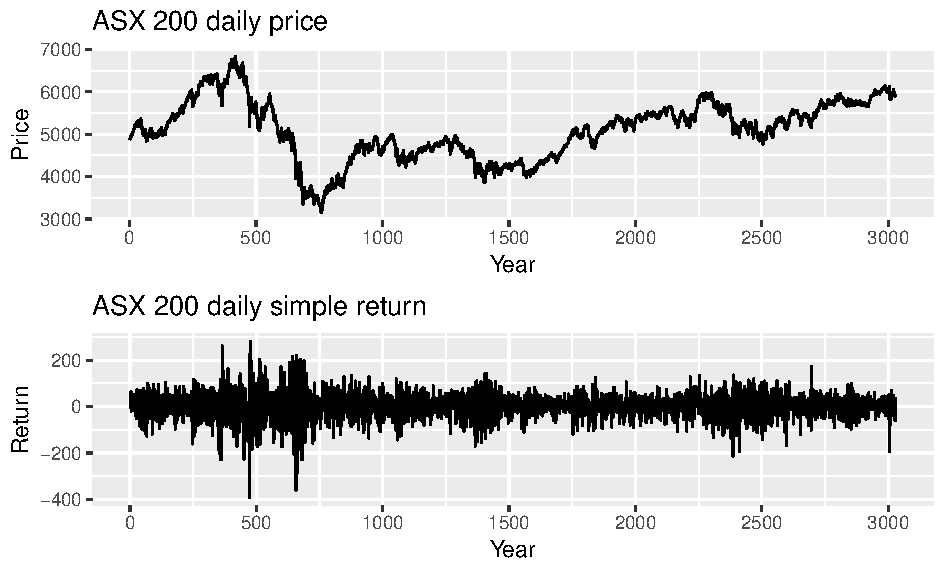
\includegraphics{thesis_files/figure-latex/asxplot-1.pdf}

In order to facilitate the final assessment, we have set the data before
2017 as train data, the data from 2017 until early 2018 as test data.
Then using train data to select suitable ARIMA model and GARCH model to
make both interval forecasts and probabilistic forecasts. For the
forecasting results, different scoring rules are used to evaluate them
respectively. Finally, compare the results of the score to evaluate the
quality of the forecast results. Because in this case study, only single
one time series is used, there is no the impact of the unit in the
comparison. Therefore, we do not have to consider any standardization
problem.

\section{Select suitable models}\label{select-suitable-models}

\subsection{ARIMA model}\label{arima-model}

For the selection of models, we first use the `auto.arima' function to
find the most suitable model. Based on the train set, the ARIMA model is
selected to be shown below.

\begin{table}

\caption{\label{tab:arima}ARIMA model select}
\centering
\begin{tabular}[t]{lr}
\toprule
  & x\\
\midrule
ma1 & -0.0398745\\
ma2 & 0.0063880\\
ma3 & -0.0504566\\
\bottomrule
\end{tabular}
\end{table}

According to table 4.1, it shows that ARIMA model does not have the
autoregressive part, and the order of the moving average part is equal
to 3. So, MA(3) model is the model what we need to use. This result is
used to continue selecting the GARCH model.

\subsection{GARCH model}\label{garch-model}

Unlike the selection of ARIMA models, there is no automatic program to
help us select the most suitable GARCH model. Therefore, we define 6
different GARCH models based on the ARIMA model, which be selected
before and then use `garchFit' function from fGarch package to estimate
them separately. According to the result, the model with minimum AIC is
chosen as the optimal model.

\begin{table}

\caption{\label{tab:table1}Garch model select}
\centering
\begin{tabular}[t]{lrrrr}
\toprule
  & AIC & BIC & SIC & HQIC\\
\midrule
garch11 & 10.608 & 10.623 & 10.608 & 10.614\\
garch12 & 10.609 & 10.626 & 10.609 & 10.615\\
garch21 & 10.609 & 10.626 & 10.609 & 10.616\\
garch22 & 10.610 & 10.629 & 10.610 & 10.617\\
arch1 & 10.779 & 10.791 & 10.779 & 10.783\\
arch2 & 10.729 & 10.744 & 10.729 & 10.734\\
\bottomrule
\end{tabular}
\end{table}

According to the result as table 4.2, the AIC of the MA(3)-GARCH(1,1) is
10.608, it is the smaller than other models. Therefore, The
MA(3)-GARCH(1,1) is considered the most suitable model for the train
set.

\section{Interval forecast for the ASX 200
index}\label{interval-forecast-for-the-asx-200-index}

For interval prediction, Winkler loss scoring rule is used. According to
its formula, the score is affected by the size of the predictive
interval. Therefore, we want to know what changes will be made in the
interval score under different predictive interval levels. First, we use
the previous MA(3) model to make the forecast. By setting 21 different
prediction intervals \((1-\alpha)\times100\%\) from 1\% to 99\%, the
results of interval forecasts at different prediction interval level are
obtained.

Because the scoring rule is to score every prediction result, to take
the average of scoring results can be easy to observe the changes as the
size of predictive interval increasing. Then the 21 scores under 21
predictive interval levels are obtained. Using them to make a curve as
the blow.

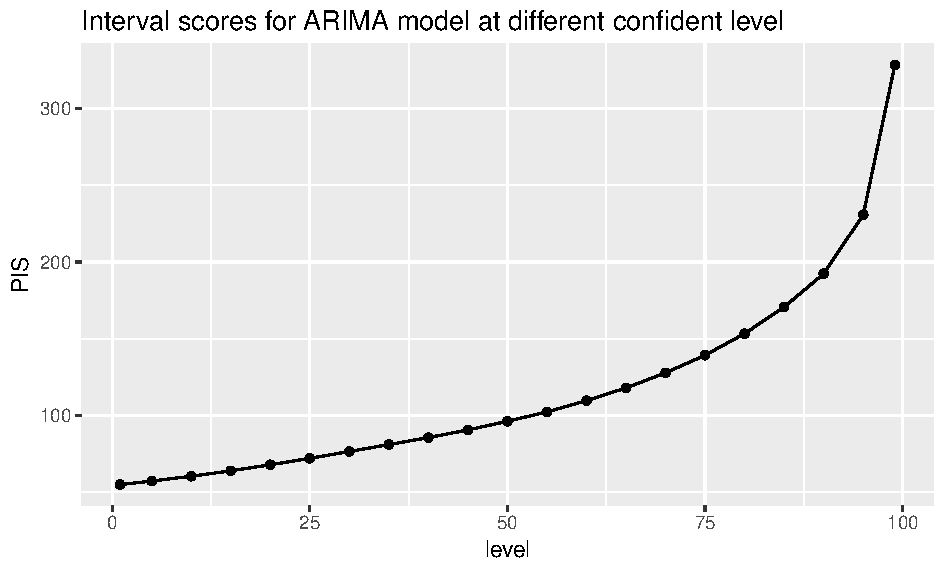
\includegraphics{thesis_files/figure-latex/plot1-1.pdf}

This graph shows that as the predictive interval increases, the interval
score shows a trend of accelerating and increasing, and the score
reaches the highest at 99\%. The lower the score represents the better
result of the interval forecasts, so the information from this curve
shows that the interval forecasts for the simple return of the ASX200 by
using ARIMA model are better when the prediction interval level is
smaller.

Then use the same way to set prediction interval levels, and use
MA(3)-GARCH(1,1) model to forecast the intervals again. The scores of
forecast results under same predictive interval are also taken average
respectively. After that, a score change curve for GARCH model is
obtained, which shows the result very similar to that obtained by using
the ARIMA model before.

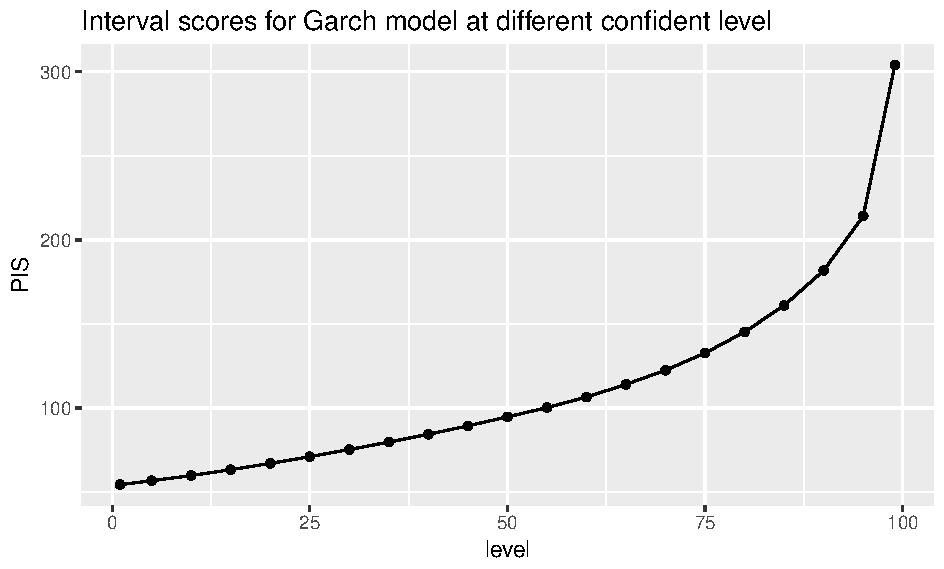
\includegraphics{thesis_files/figure-latex/plot2-1.pdf}

This graph also shows that as the prediction interval expands, the score
increases. It means that the smaller prediction intervals show better
score results by using MA(3)-GRACH(1,1) model. Because the images
produced by using the two different models are extremely similar, we put
them together for comparison.

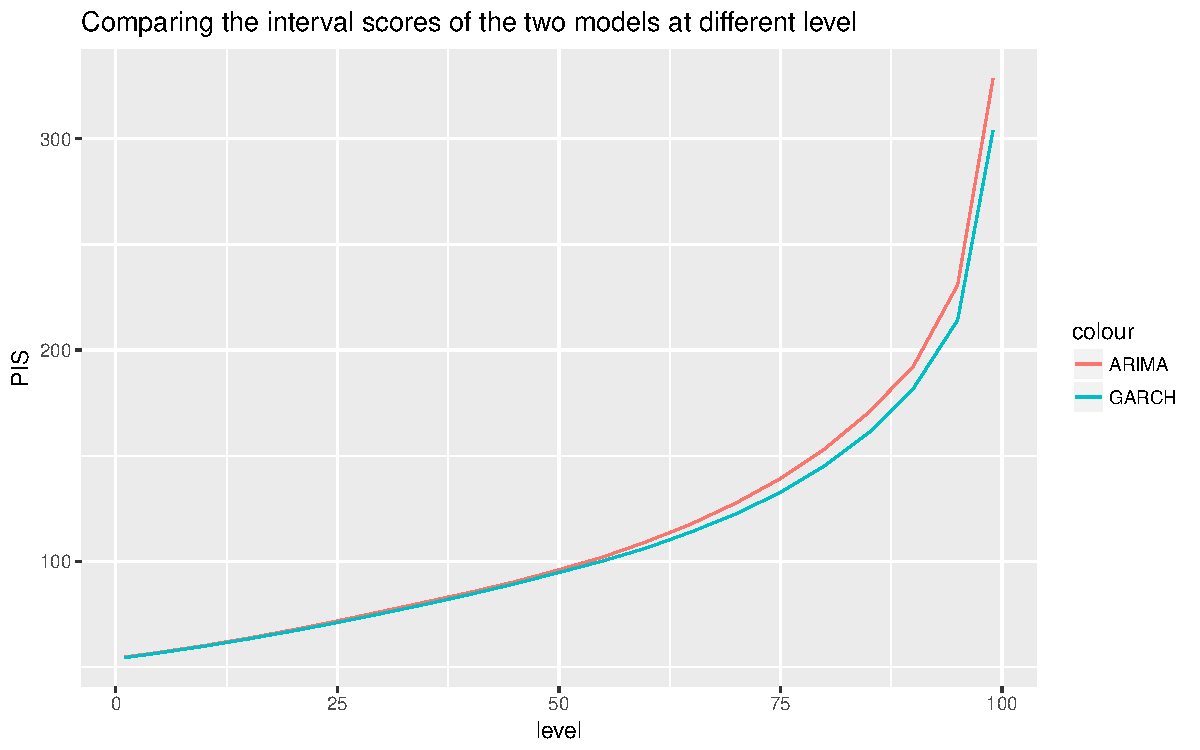
\includegraphics{thesis_files/figure-latex/plot3-1.pdf}

By comparing these two curves, their overall characteristics are
extremely similar. Their scores are not very different at smaller
predictive intervals level, but in the larger prediction interval level,
the scores are slightly different by using these two different models.
The interval scores of interval forecasts by using MA(3)-GRACH(1,1)
model is becoming smaller than that by using MA(3) model as the
prediction interval expands. So, at high predictive interval level,
interval forecasts by using GARCH model has a relatively good
performance. This result illustrates, for the interval forecast of
financial return time series, GARCH model can provide the more efficient
result to forecasters. And it is also proving that it is more suitable
for fitting financial data.

\section{Probabilistic forecasts for the ASX 200
index}\label{probabilistic-forecasts-for-the-asx-200-index}

For probabilistic forecasts, we still using the ARIMA(0,0,3) model and
MA(3)-GARCH(1,1) model to fit data and make a forecast, which was
produced at section 4.1. However, unlike the result obtained in section
4.2, we do not need to set the predictive interval. Instead, we use the
functions of `logs\_norm', `crps\_norm' and `dss\_norm' from
``scoringRules'' package (\textcite{JKL17}) in R to directly calculate
the scores, and these three functions represent these three distribution
scoring rules under Gaussian predictive distribution: Logarithmic score,
Continuous Ranked Probability Score and Dawid-Sebastianti score.

\begin{table}

\caption{\label{tab:table2}Scoring Rules for MA model and GARCH model}
\centering
\begin{tabular}[t]{lrrr}
\toprule
  & CRPS & LogS & DSS\\
\midrule
GARCH & 20.70 & 5.10 & 8.36\\
ARIMA & 21.13 & 5.14 & 8.45\\
\bottomrule
\end{tabular}
\end{table}

For the scores by using the same model and the same score rule, we also
get their mean. Then table 4.3 is generated. According to this table,
the scores of three type scoring rules of MA(3)-GARCH(1,1) model are all
smaller than the result of MA(3) Model. This result shows that for the
selected financial time series (ASX 200), the GARCH model can get better
prediction results than the ARIMA model.

By observing all the previous results, no matter for interval prediction
or probability prediction, the Garch model all can have a better
performance than the ARIMA model, although it prediction effect under
the high predictive interval level is much worse than that in the low
predictive interval. This result also shows that compared with the ARIMA
model, the GARCH model can analyze and predict the financial data more
accurately.

\chapter{Case study two: M3 datasets}\label{case-study-two-m3-datasets}

The M3 dataset includes 3003 different type time series, it is from R
packages ``Mcomp'' (\textcite{RH182}). These time series are from
different fields, so their data units are different. Base on the time
type, they can be divided into three large classes, yearly data monthly
data and quarterly data. For each time series, there are a train set and
a test set, which can be easily used to build each forecast models, then
predicting and scoring. Different from previous financial data, M3
datasets can use different models for predictive analysis at the same
time. Therefore, it can provide more information for evaluating
forecasts by using scoring rule.

As in the previous chapter, before we start forecasting and evaluating,
the suitable models should be selected. In this case study, three
prediction models are chosen, ARIMA model, ETS model, and Random walk
model. However, for the M3 datasets, there are more than 3000 different
time series, so we have modelled all the time series separately by using
these three models.

Before the analysis of the M3 dataset, there is a problem that needs to
be noticed. These different time sequences come from different fields
and their units are different. As we discussed in the second chapter, it
is necessary to standardize each scoring result by using Winkler loss
scoring rule and continuous ranked probability Scoring rule. If data are
not standardized, the final result will be the mistake.

\section{Model selection}\label{model-selection}

As in the previous chapter, before we start forecasting and evaluating,
the suitable models should be selected. In this case study, three
prediction models are chosen, ARIMA model, ETS model, and Random walk
model. However, for the M3 datasets, there are more than 3000 different
time series, so we have modelled all the time series separately by using
these three models. The three models can be selected by the automatic
program, which is introduced in the third chapter. Then they can be used
for interval prediction or probability prediction. So there is no more
detailed discussion here.

\section{Interval forecast for the M3 competition
data}\label{interval-forecast-for-the-m3-competition-data}

Like case study one, firstly, we need to use the optimality model
selected by automatic programs to predict interval for all time series
from M3 datasets. Then use Winkler loss scoring rule to score each
prediction result. The difference is that we no longer need to observe
the impact of the different prediction interval level on the interval
prediction results, so we did not set different predictive interval
levels. Instead, all of the interval forecasts are under the 95\%
prediction interval. Each scoring results for every time series by
evaluating forecasts, we also take their mean as the final result.

It should be noted that after getting the interval score, we need to use
the scores by assessing the forecasts of random walk model to
standardize the results from ARIMA and ETS model, to remove the impact
of units from different time series.

\[Standardized~interval~score=\frac{Interval~scores~for~ARIMA~model~or~ETS~model}{Interval~scores~for~RW~model}\]

Then use the standardized scores to produce the graph to compare the
results. Here we use box plot, which an intuitively identify outliers in
data sets and determine the degree of dispersion and bias in data sets.
Also, use the different box plot to compare the scoring results from
time series under different time types. Then the box plots are
generated.

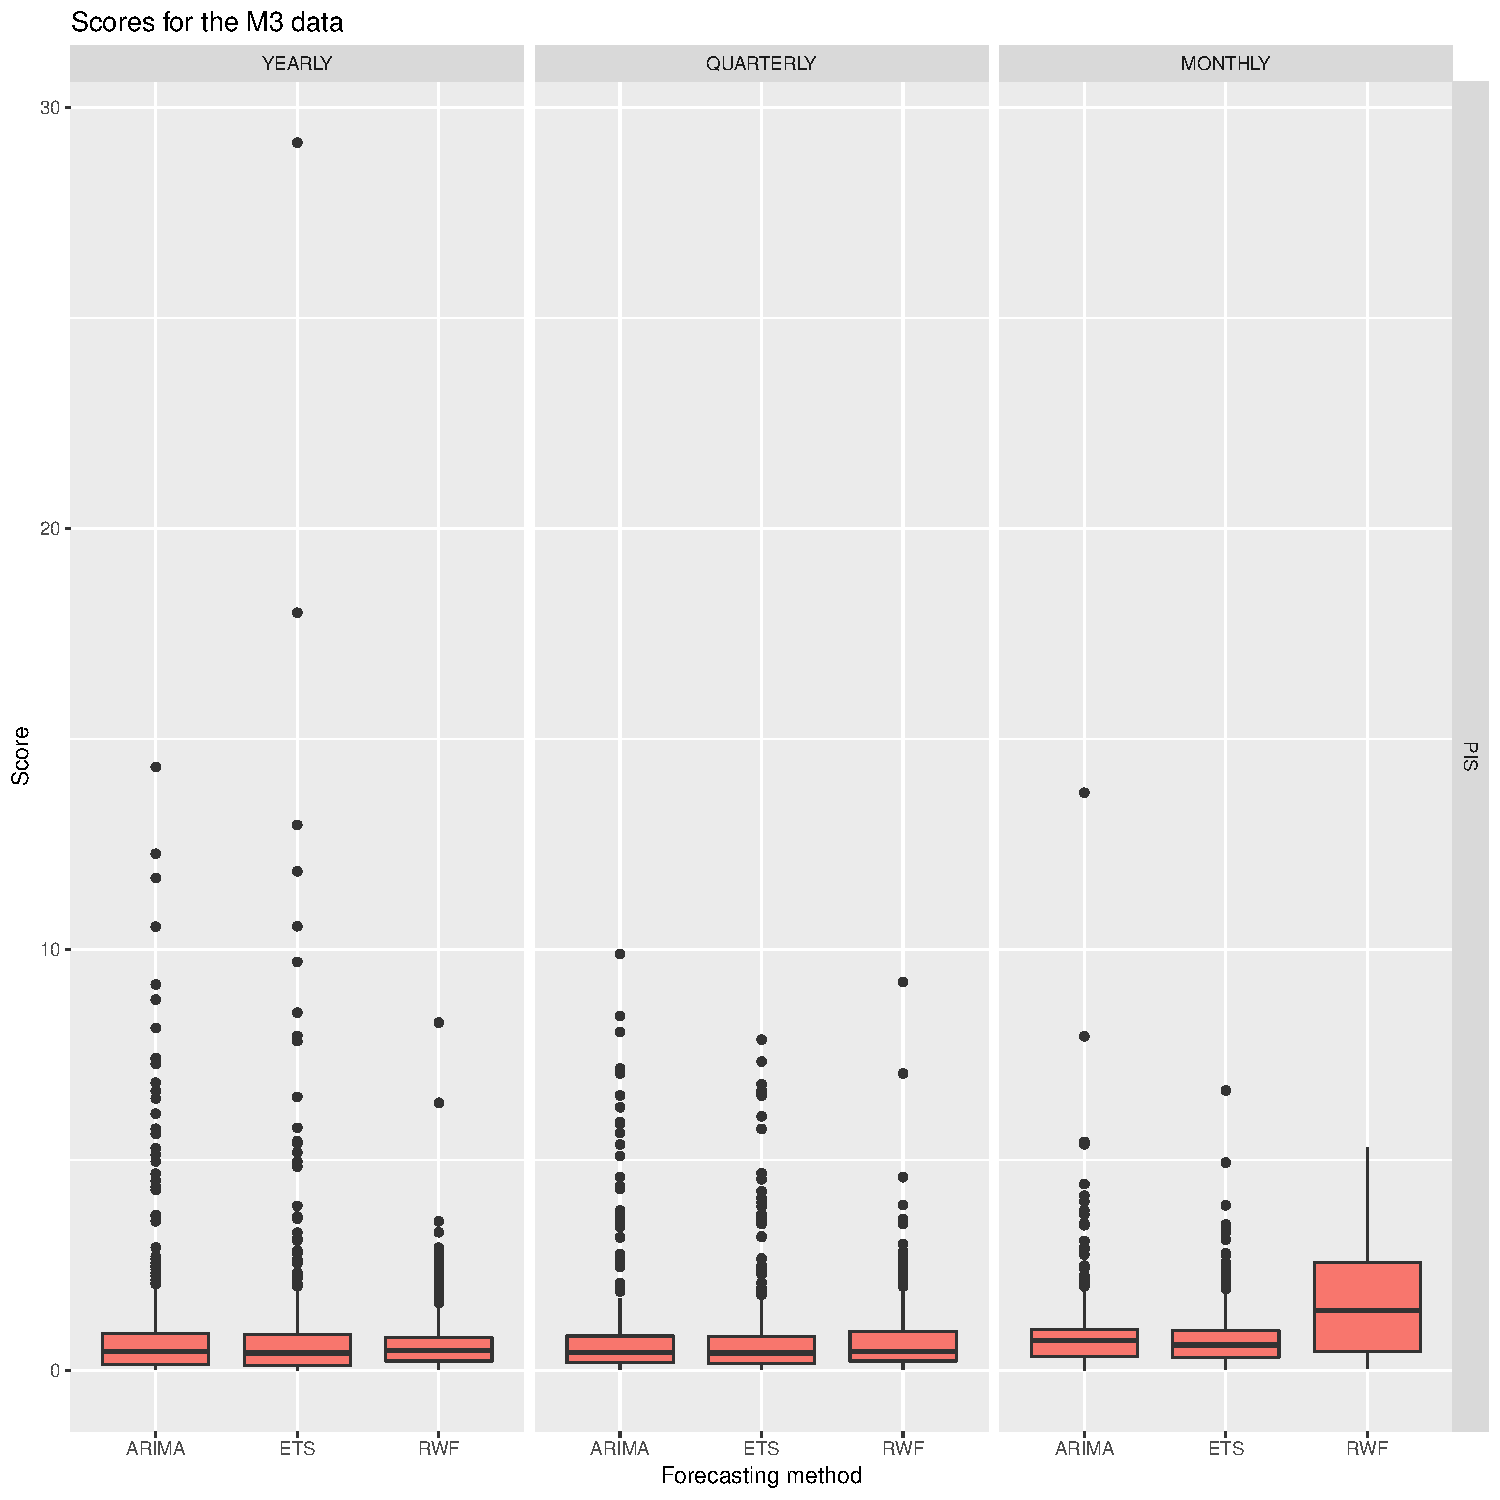
\includegraphics[width=1\linewidth]{thesis_files/figure-latex/boxplotPIS-1}

According to the whole box plots, we can not see clearly which model has
better interval prediction results. However, it can be seen that quite a
number of outliers are displayed over 95th percentile line. This shows
that comparing the standard normal distribution, the score distribution
shows that the tail is too heavy, and the degree of freedom is small.
Because the outliers are concentrated on one side of the larger value,
the distribution appears right-biased. The reason for this result is
that the scores based on Winkler loss scoring rule formula are always
greater than or equal to the difference between upper and lower
endpoints. ALsoThe scores of the ETS model are lower than those of the
ARIMA model at 5th, 25th, 50th, 75th and 95th percentiles, whether they
are from monthly data or quarterly data for yearly data.

In order to observe the results more clearly, we produce the box plots
on the log scale.

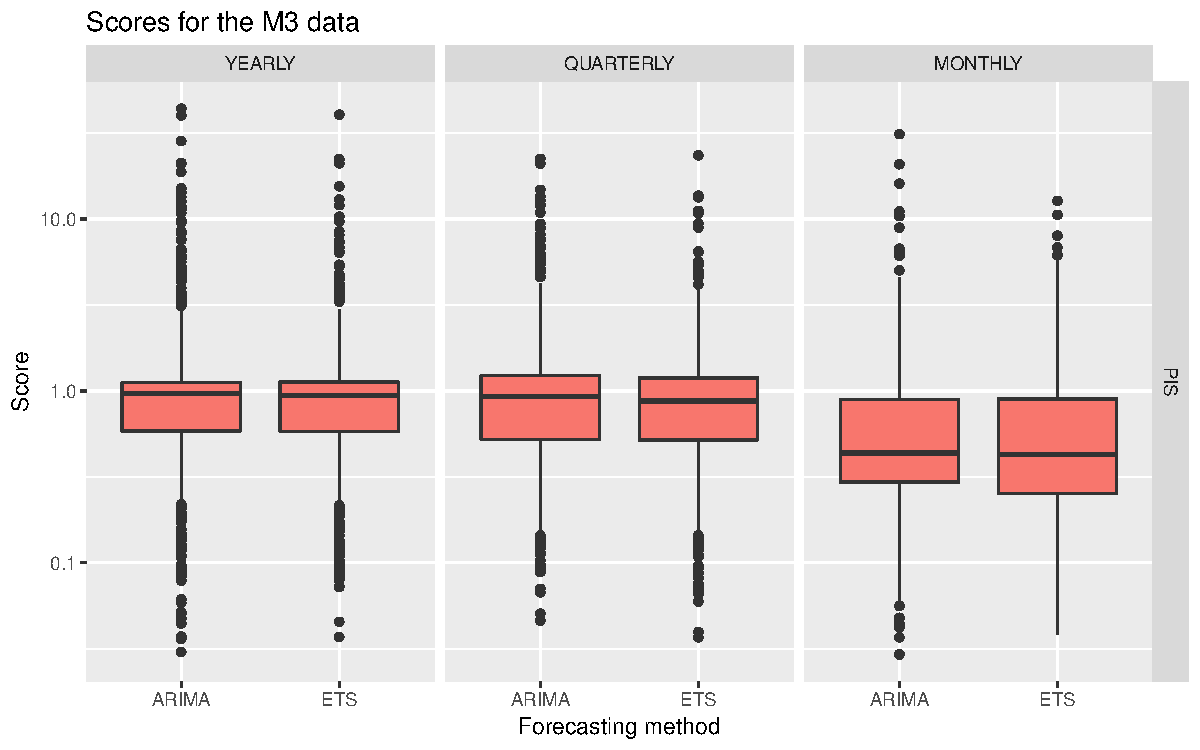
\includegraphics[width=1\linewidth]{thesis_files/figure-latex/boxplotlogPIS-1}

This is the result boxplot of interval scores on the log scale. The
boxplots can show 5th, 25th, 50th, 75th and 95th percentiles of central
prediction interval width. And for the yearly and quarterly time series,
the interval scores are similar by the different model, only the line at
the 50th percentile for ETS model shows a bit lower than that for ARIMA
model. So we consider that ETS model has better prediction performance
to make interval forecasts for the yearly and quarterly time series. For
monthly data, the score results show a great difference. The line at the
25th percentile of ETS model is clearly lower than that of ARIMA model.
And the distance between the upper and lower limits of ETS model is
obviously greater than ARIMA. This shows that for the monthly time
series ETS score has great volatility and is not very concentrated, so
the prediction result of ETS model is not as good as ARIMA model. The
forecasts by ARIMA model have the sharper sharpness and the calibration
is more accurate,

\section{Probabilistic forecasts for the M3 competition
data}\label{probabilistic-forecasts-for-the-m3-competition-data}

In this part, we make the probabilistic forecasts of each time series by
using the same time series models as before. However, the scoring rules
will use the distribution scoring rules. It is important to note that,
as previously discussed in the second chapter, although the logarithmic
score and Dawid-Sebastianti score will directly transform the data so
that the results should not standardized. But, when the continuous
ranked probability score is used, the scoring results need to be
standardized. The standardization method is the same as the method to
deal with the interval prediction.

\[Standardized~CRPS~score=\frac{CRPS~scores~for~ARIMA~model~or~ETS~model}{CRPS~scores~for~RW~model}\]

After the probabilistic forecasts from each time series has been scored
by three distribution scoring rules, and the scores have been taken the
average, we get the final scoring results. Certainly, the results by
using the CRPS scoring rules should be standardized. Using the same way
of the interval score, we get the box plot with different scoring rules
under different time types. The original image is shown next page.

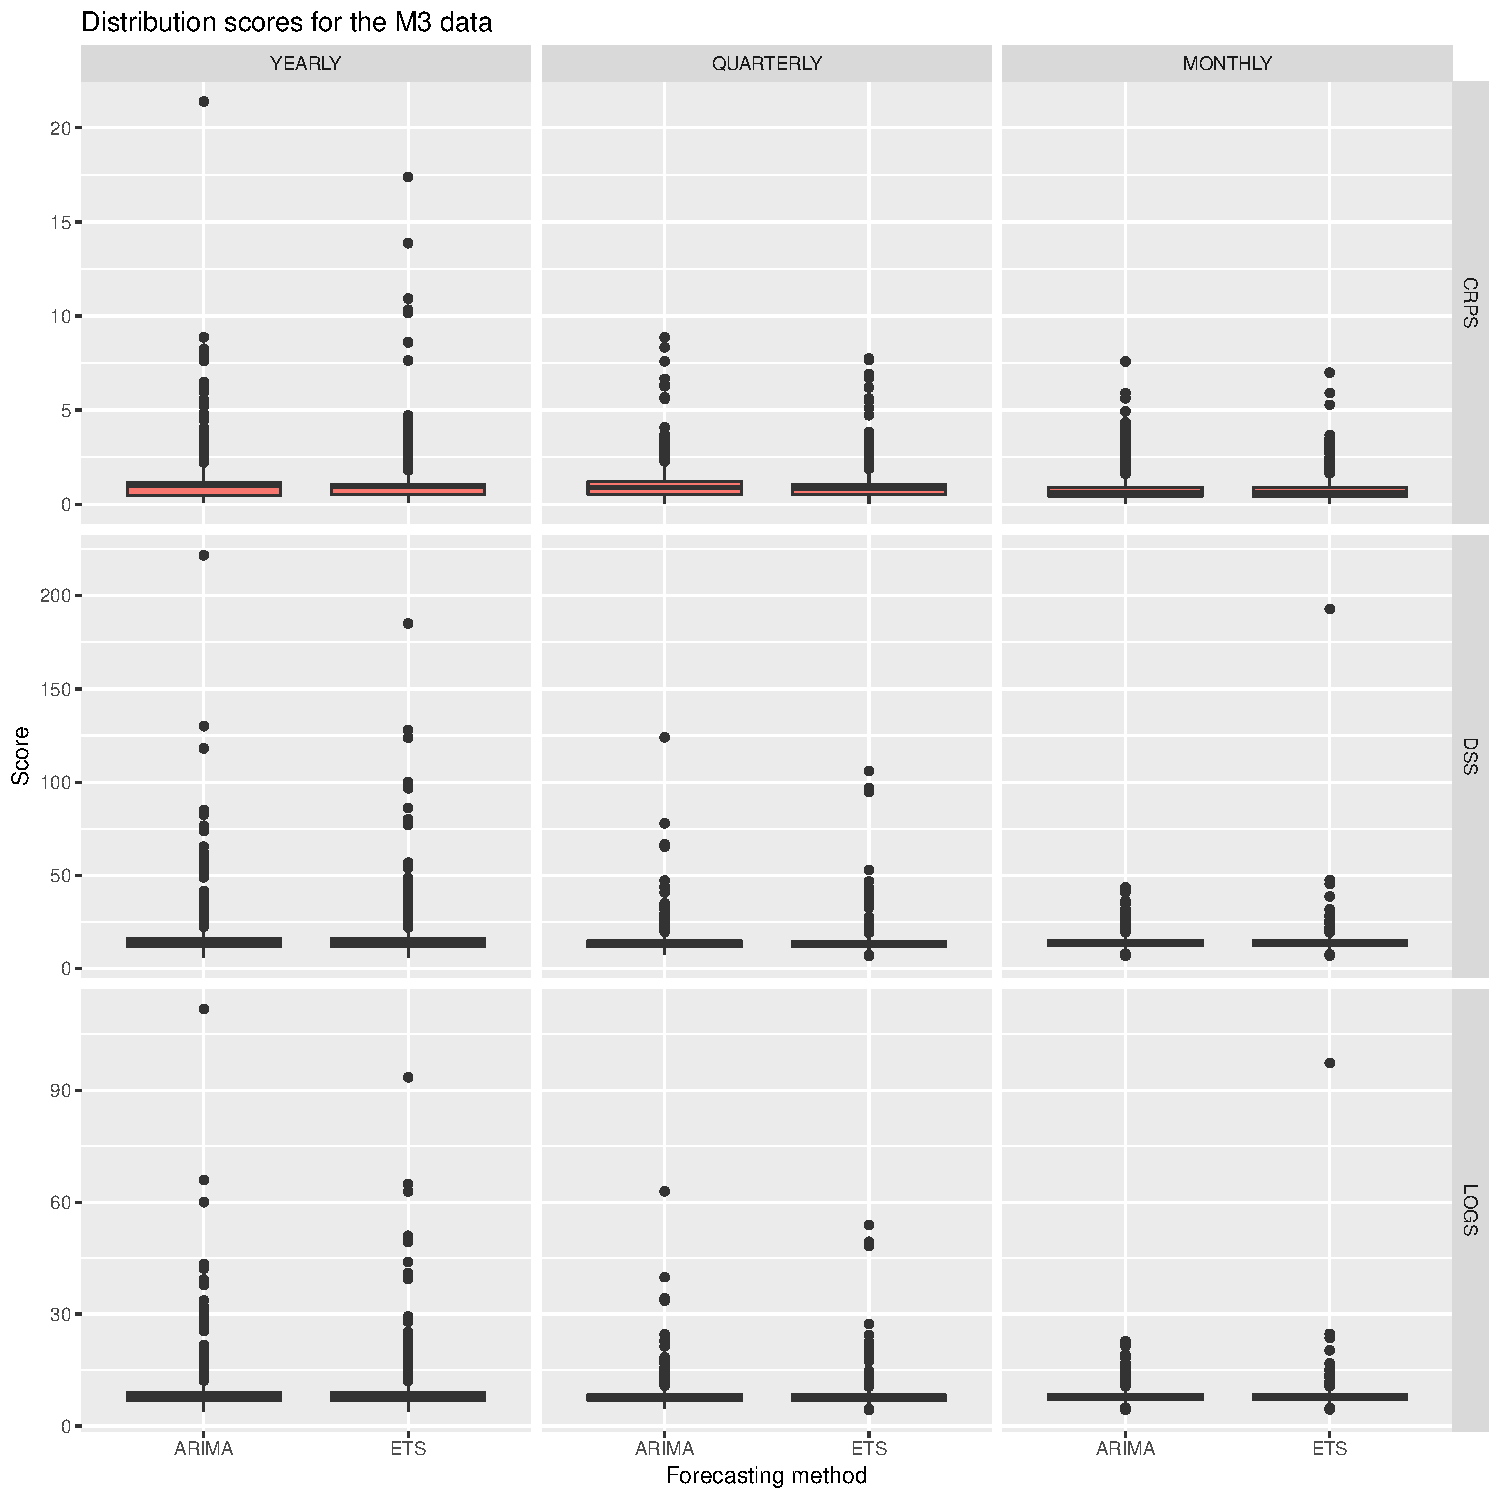
\includegraphics[width=1\linewidth]{thesis_files/figure-latex/boxplot-1}

According to the information of these box plots, we are hard to
distinguish which model is better for making probabilistic forecasting
under different time types of time series. But these plots are still
clearly displayed that the most outliers are concentrated over the 95th
percentile. This shows that the tail of the score distribution is heavy
and the distribution is right-skewed.

In order to display the results more clearly, we have also processed
this figure, to produce the boxplots on the log scale.

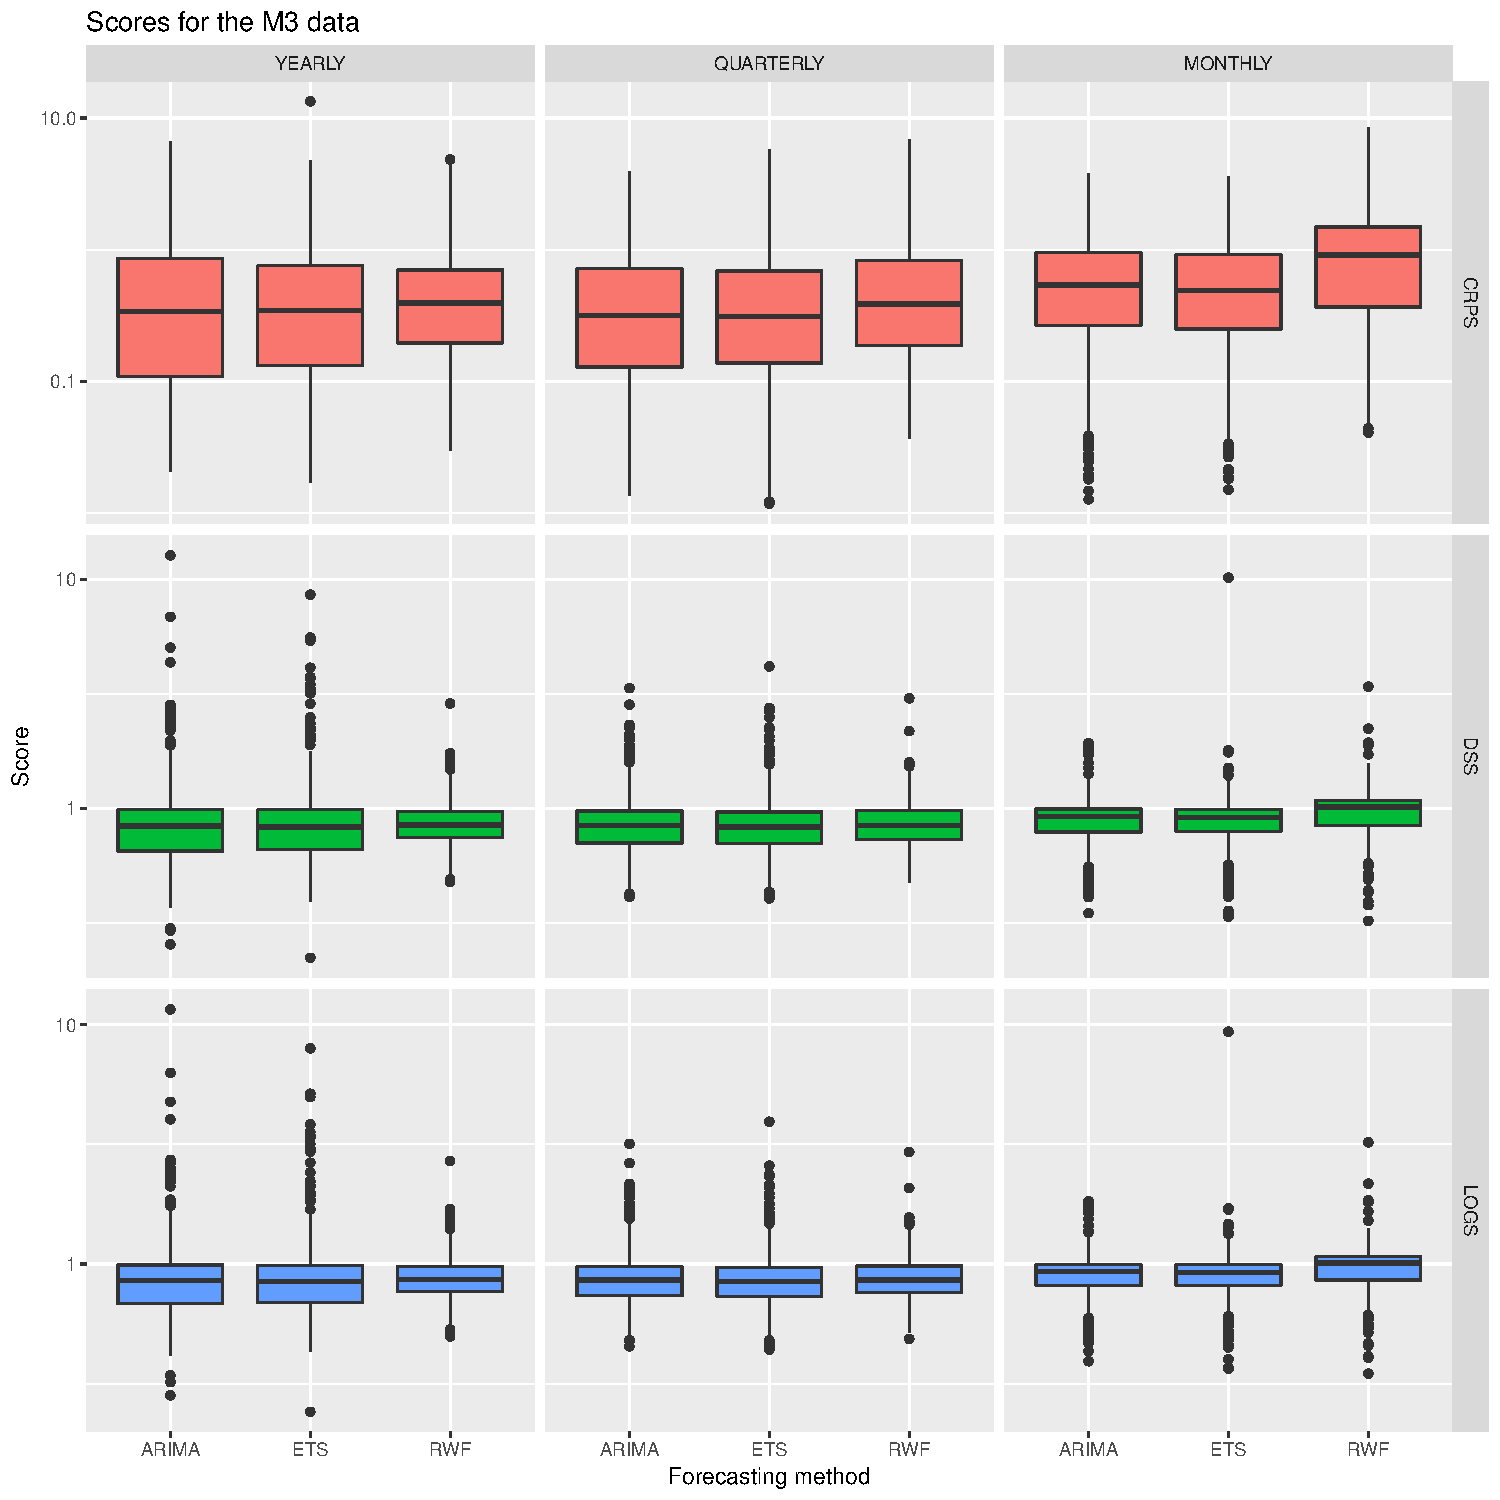
\includegraphics[width=1\linewidth]{thesis_files/figure-latex/boxplotlog-1}

According to this graphs, where CRPS scoring rules are used, the
prediction scores for all time types of time series show that the ETS
model has better prediction sharpness, because the distance between his
upper and lower limits, and distance of the 25th percentile and 75th
percentile lines are all small than the distances of the ARIMA model.
Although the median lines from this two model are almost equal, we still
think ETS models have the better predictive performance by using CRPS
scoring rules.

For score results by using LogS and DSS scoring rules, although the
differences shown in the box plots are not particularly large, we can
still see that the score distribution of the ETS model is more
concentrated. It indicates that the sharpness of probabilistic
prediction of ETS model is sharper. Therefore, the score results by
using LogS and DSS scoring rules also show that ETS models have the
better probabilistic predictive performance for the time series from M3
datasets.

\chapter{Conclusion and future
discussion}\label{conclusion-and-future-discussion}

\section{Conclusion}\label{conclusion}

As a common means to evaluate interval prediction and probability
prediction, scoring rules are widely used. The score of the prediction
is scored by evaluating the sharpness of the prediction result and the
calibration. This article presents two different types of scores,
interval scores and distribution scores. Interval scores are used to
score interval predictions, commonly used by Winkler loss scoring rule.
According to its formula, this scoring rule is based on whether
observations are given a rating within the prediction interval, if the
observation misses the interval, the score will depend on \(\alpha\).
For distribution scores, this paper mainly selects three scoring rules,
Logarithmic score rules, Continuous Ranked Probability Score and
Dawid-Sebastianti score. This article uses them all based on Gaussian
prediction distribution LogS and DSS scoring rules can directly transfer
data because of its own formula, so you don't have to worry about
standardization when using it. While for the CRPS scoring rule, although
it is necessary to pay attention to the standardized result when it is
used and it is difficult to evaluate the prediction result with a
complicated distribution, it can be easily used because it does not need
too much consideration of the characteristics of the prediction
distribution. Another concept that needs attention is the difference
between the confidence interval and the prediction interval, which are
often mistaken for the same. What is used when predicting using the
predictive model is the prediction interval.

Regarding the prediction model used, because different data were used in
the two case study, different models were used in the different case
study. For case study one using financial data, the ARIMA model that can
be used to analyze and forecast stationary time series, and the GRACH
model that can well explain the volatility clusters characteristics of
financial time series are used. In case study 2, because the M3 dataset
has a large number of time series in different fields, multiple types of
time series models can be used. However, because of this,
standardization issues need to be noted when comparing the final score
results. Here ARIMA, ETS and random walk models are used.

Through the summary of case study one, the scoring rules were used to
evaluate the univariate financial time series. After evaluating the
results of the interval prediction and probability prediction generated
by the two different models, I found that comparing the results by using
ARIMA model, the GARCH model has good performance both in interval
prediction and probabilistic prediction. However, in the interval
prediction, the score obtained by the same GARCH model is high in the
case of high prediction interval level, indicating that its prediction
result is not ideal. At the low prediction interval level, it has a good
performance. For case study two, we mainly understand how to use scoring
rules to evaluate the prediction results of different types of time
series. Through the use of an automatic model-finding program, all time
series in the M3 datasets were modelled and predicted separately, and
then different prediction rules were used to evaluate separately by
using different scoring rules. For the results, both the interval
prediction and the probability prediction, the two models used for
comparison have a similar prediction performance. According to the
results of the scores, there is not a big difference in the predictions
they provide, and their appearances have their own advantages in
different predictions.

The predictive model typically provides an estimate of the forecast
distribution for each forecast range, or at least one forecast interval.
As a means to assess the accuracy of the prediction results, the scoring
rules can be intuitively given a numerical rating result for the
prediction results. Especially in applications for probabilistic
prediction, the scoring rules can simultaneously evaluate the predicted
distribution sharpness and calibration. The predictors can use these
results to determine whether the prediction results are reliable and
whether the selected prediction model is appropriate.

\section{Future discussion}\label{future-discussion}

For probabilistic prediction and interval prediction, univariate time
series are mainly used for analysis and prediction. However, in many
cases, the development of an event is not only influenced by its own
changes, but other events also affect the observed events. Therefore, it
is important to study the multivariate time series model and use this
model to make interval and probability prediction. At the same time, we
need to study new scoring rules for this situation to evaluate the
accuracy of the prediction.

\printbibliography[heading=bibintoc]



\end{document}
